\section{Experimental results}%
\label{sec:experimental_results}
%
\begin{figure*}[ht]
  \centering
  \begin{subfigure}{0.33\linewidth}
    \centering
    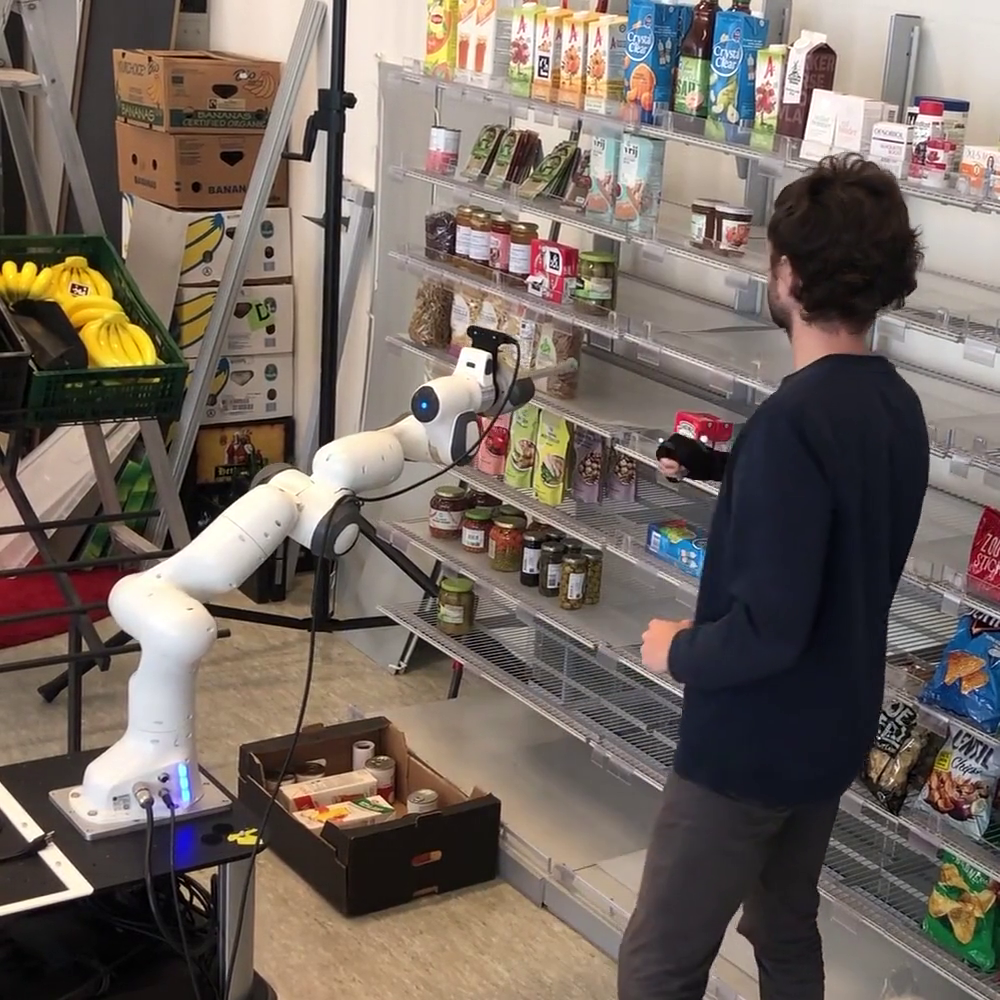
\includegraphics[width=0.9\textwidth]{3_moving_obstacles/realPanda/dynamic_fabrics_optitrack_1.png}
    \caption{$t=0$s}%
    \label{subfig:experiment3_realPanda_example_1}
  \end{subfigure}%
  \begin{subfigure}{0.33\linewidth}
    \centering
    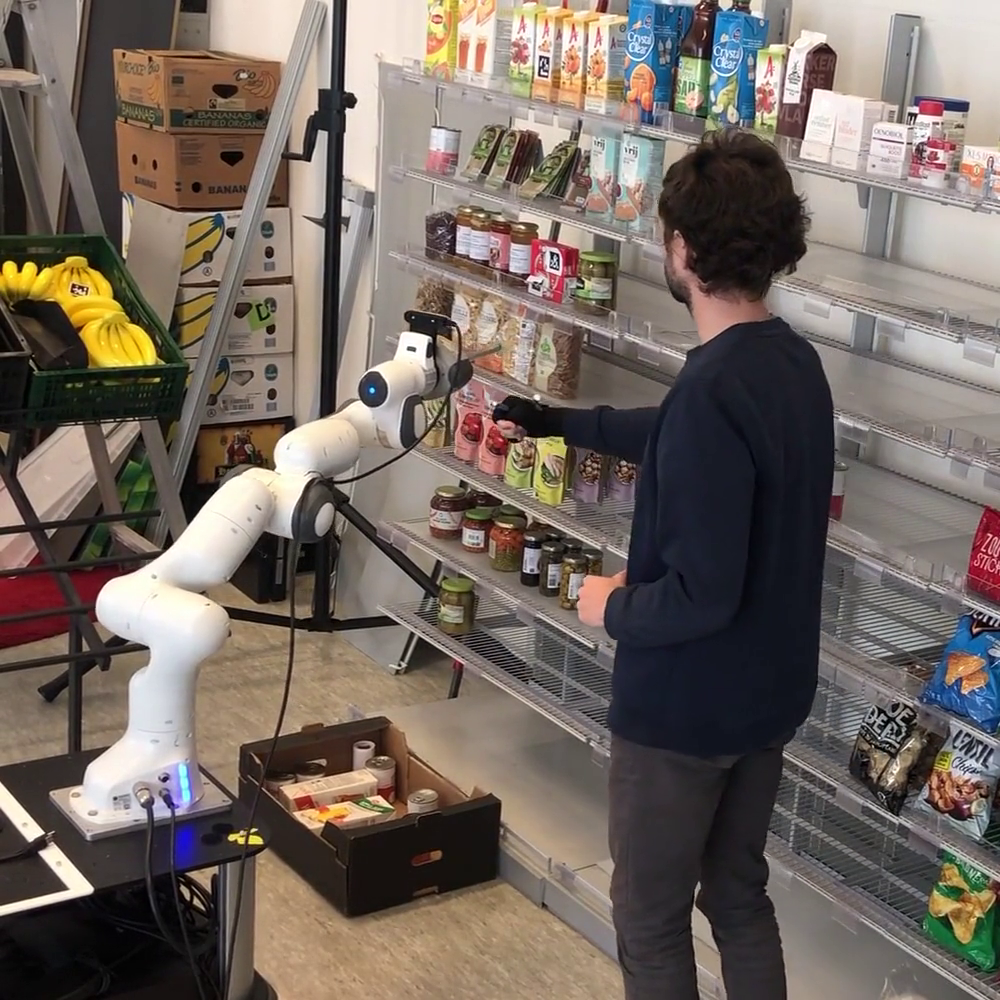
\includegraphics[width=0.9\textwidth]{3_moving_obstacles/realPanda/dynamic_fabrics_optitrack_2.png}
    \caption{$t=2$s}%
    \label{subfig:experiment3_realPanda_example_1}
  \end{subfigure}%
  \begin{subfigure}{0.33\linewidth}
    \centering
    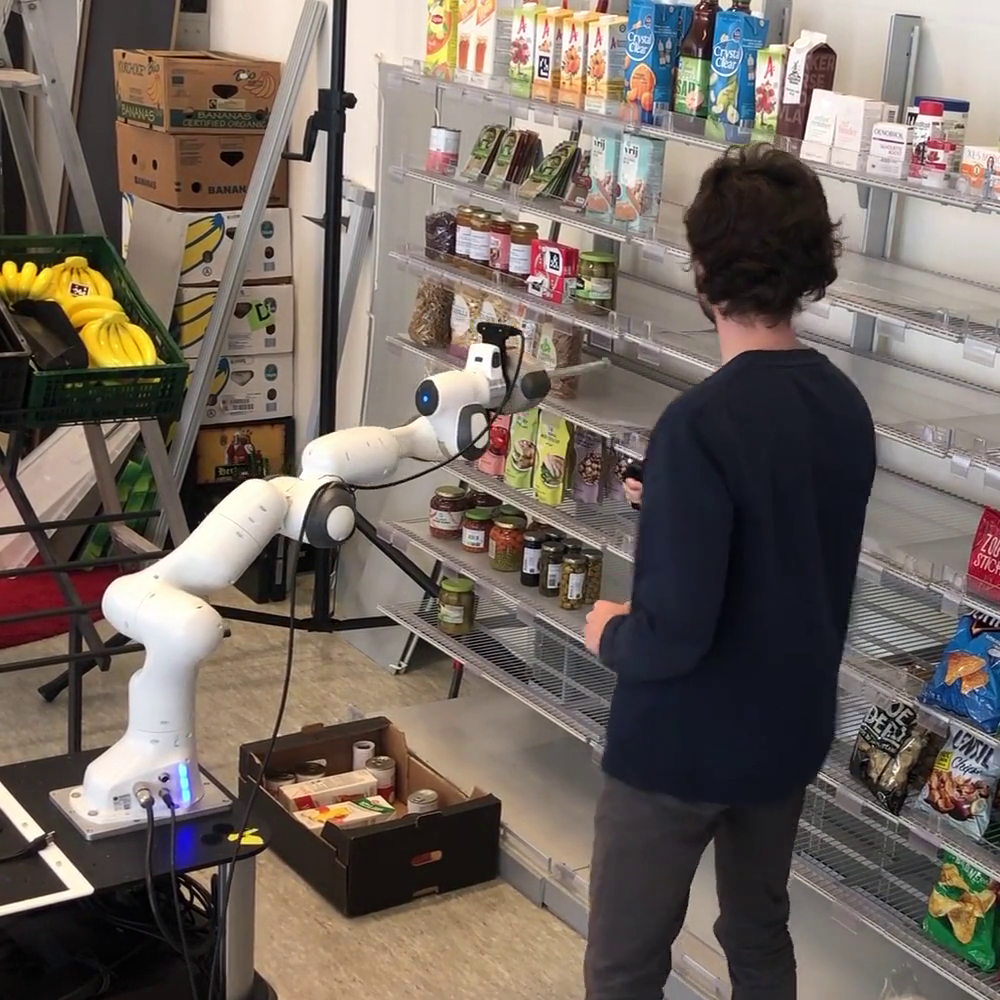
\includegraphics[width=0.9\textwidth]{3_moving_obstacles/realPanda/dynamic_fabrics_optitrack_3.png}
    \caption{$t=3$s}
    \label{subfig:experiment3_realPanda_example_1}
  \end{subfigure}%
  \caption{\acl{df} in the presence of a human. The human hand's state is estimated with a motion capture
    system. The robot smoothly and in advance avoids the human operator and allows for safe coexistence.
  }%
  \label{fig:experiment6_realPanda}
\end{figure*}

In this section, the performance of optimization fabrics is assessed on various
robotic platforms. Although~\cite{Ratliff2020} suggested performance benefits
over optimization-based methods to local motion planning, no quantitative
comparisons have been presented to this date. 
The scenarios that we have chosen here (especially in the 
first two experiments) are intentionally simple to identify the specific
differences. In the real world experiments, we show the differences
on more dynamic scenarios, where the limited frequency of a global
planning method, such as RRT, justifies the need for a local planning method.
To give a general idea of the
performance differences between \ac{sf} and receding-horizon trajectory
optimization, we compare the performance of an \ac{mpc} formulation, adapted
from~\cite{Spahn2021}, with \ac{sf}, as proposed in~\cite{Ratliff2020}.  The
second experiment compares performance between \ac{sf} and \ac{df} for
trajectory following tasks. In the third experiment, moving obstacles are added
to the scene to form a dynamic environment. Our extension to non-holonomic
systems is tested in the fourth experiment. Then, everything is combined in
an experiment with a differential drive mobile manipulator.
Finally, we present a possible application of a robot sharing the environment
with a human.
The experiments described here are supported by videos accompanying this paper.

\subsection{Settings \& performance metrics}%
\label{sub:settings}

We present a detailed analysis of the experimental results for two commonly used setups,
namely the \textit{Franka Emika Panda}, a \textit{Clearpath Boxer}, and a mobile manipulator
composed of both components
see~\cite{Spahn2021}. Note, that these
robots are representative of commonly used robots in dynamic environments. The
Franka Emika Panda is a 7 degree-of-freedom robot with joint torque sensors, comparable to the
Kuka Iiwa. Mobile manipulators equipped with differential drives are widely used by other
manufacturers, see Pal Robotics Tiago or the Fetch Robotics Mobile Manipulator.
%Results on simpler kinematic chains can be found in
%\cref{app:sec:complete_list_of_experiments}.

Compared to~\cite{Cheng2018}, we propose a more extensive list of metrics.
With regards to safety, we measure the \textbf{Clearance}, the minimum distance
between the robot and any obstacle along the path.
%Moreover, \textbf{Self-Clearance} is defined as the minimum distance between
%any two links of the robot.
For static goals, solver planner performance is measured in terms of
\textbf{Path Length}, euclidean length of the end-effector trajectory, and
\textbf{Time-to-Goal}, time to reach the goal. For trajectory following tasks,
this measure\ is replaced by \textbf{Summed Error}, the normed sum of deviation
from the desired trajectory. Computational costs are measured by the average
\textbf{Solver Time} in each time step. Most important, binary success is
measured by the \textbf{Success Rate}, where failure indicates that either the
goal was not reached or a collision occurred during execution. Performance
metrics are only evaluated if the concerned motion generator succeeded.
More information on the testbed can be found in \cite{spahn2022local}.
 
In static, industrial environments the time to reach the goal can be considered
the one single most important metric, but we argue that dynamic environments
require a more nuanced performance evaluation and thus a set of metrics.
Intentionally, we do not give general weights to the individual metrics, as
their corresponding importance highly depends on the application. As a
consequence, we tuned the compared planners in such a way that they reach the
goal in a similar time. Note that the general speed for all planners compared
in this article can be adjusted by choosing a different parameter setup.

As this work does not focus on obstacle detection, we simplify
obstacles to spheres. Thus, we assume that an operational perception
pipeline detects obstacles and constructs englobing spheres.
The experiments are randomized in either the location of the obstacles, the location of the
goal, the initial configuration, or in a combination of all three aspects.
For every experiment, the type and level of randomization are stated.

\subsection{Experiment 1: Static fabrics vs. \ac{mpc}}%
\label{sub:experiment_1_static_fabrics_vs_mpc}

In the first experiment, we compare the performance of an \ac{mpc}
formulation with \ac{sf}
\cite{Ratliff2020,Wyk2022}.
%
Compared to the formulation used in \cite{Spahn2021}, we use a workspace goal
rather than a configuration space goal, and apply a second order integration
scheme so that the control outputs are accelerations instead of velocities. We
clarify that the formulation deployed for the following tests is geometric as
the model used is a second order integrator and does not include the dynamics
of the robots. The main reason lies in the reduced computational costs and the
inaccessibility of a highly accurate model \cite{meo2021adaptation}.

\paragraph{Parameters}
The low-level controller of the robot runs at $1$ kHz. The fabrics are running at $100$ Hz
and the \ac{mpc} at $10$ Hz. The time horizon for the \ac{mpc}
planner was set to $T=3$s spread equally over
$H=30$ stages. Based on the findings in~\cite{Spahn2021}, we are confident that the \ac{mpc}
planner is close to its optimal settings. Moreover, we used the implementations
by~\cite{forcespro,forcesnlp}, which are reported to have improved performance over
open-source libraries like \textit{acado}.

\begin{figure}[h]
  \centering
  \begin{subfigure}{0.4\linewidth}
    \centering
    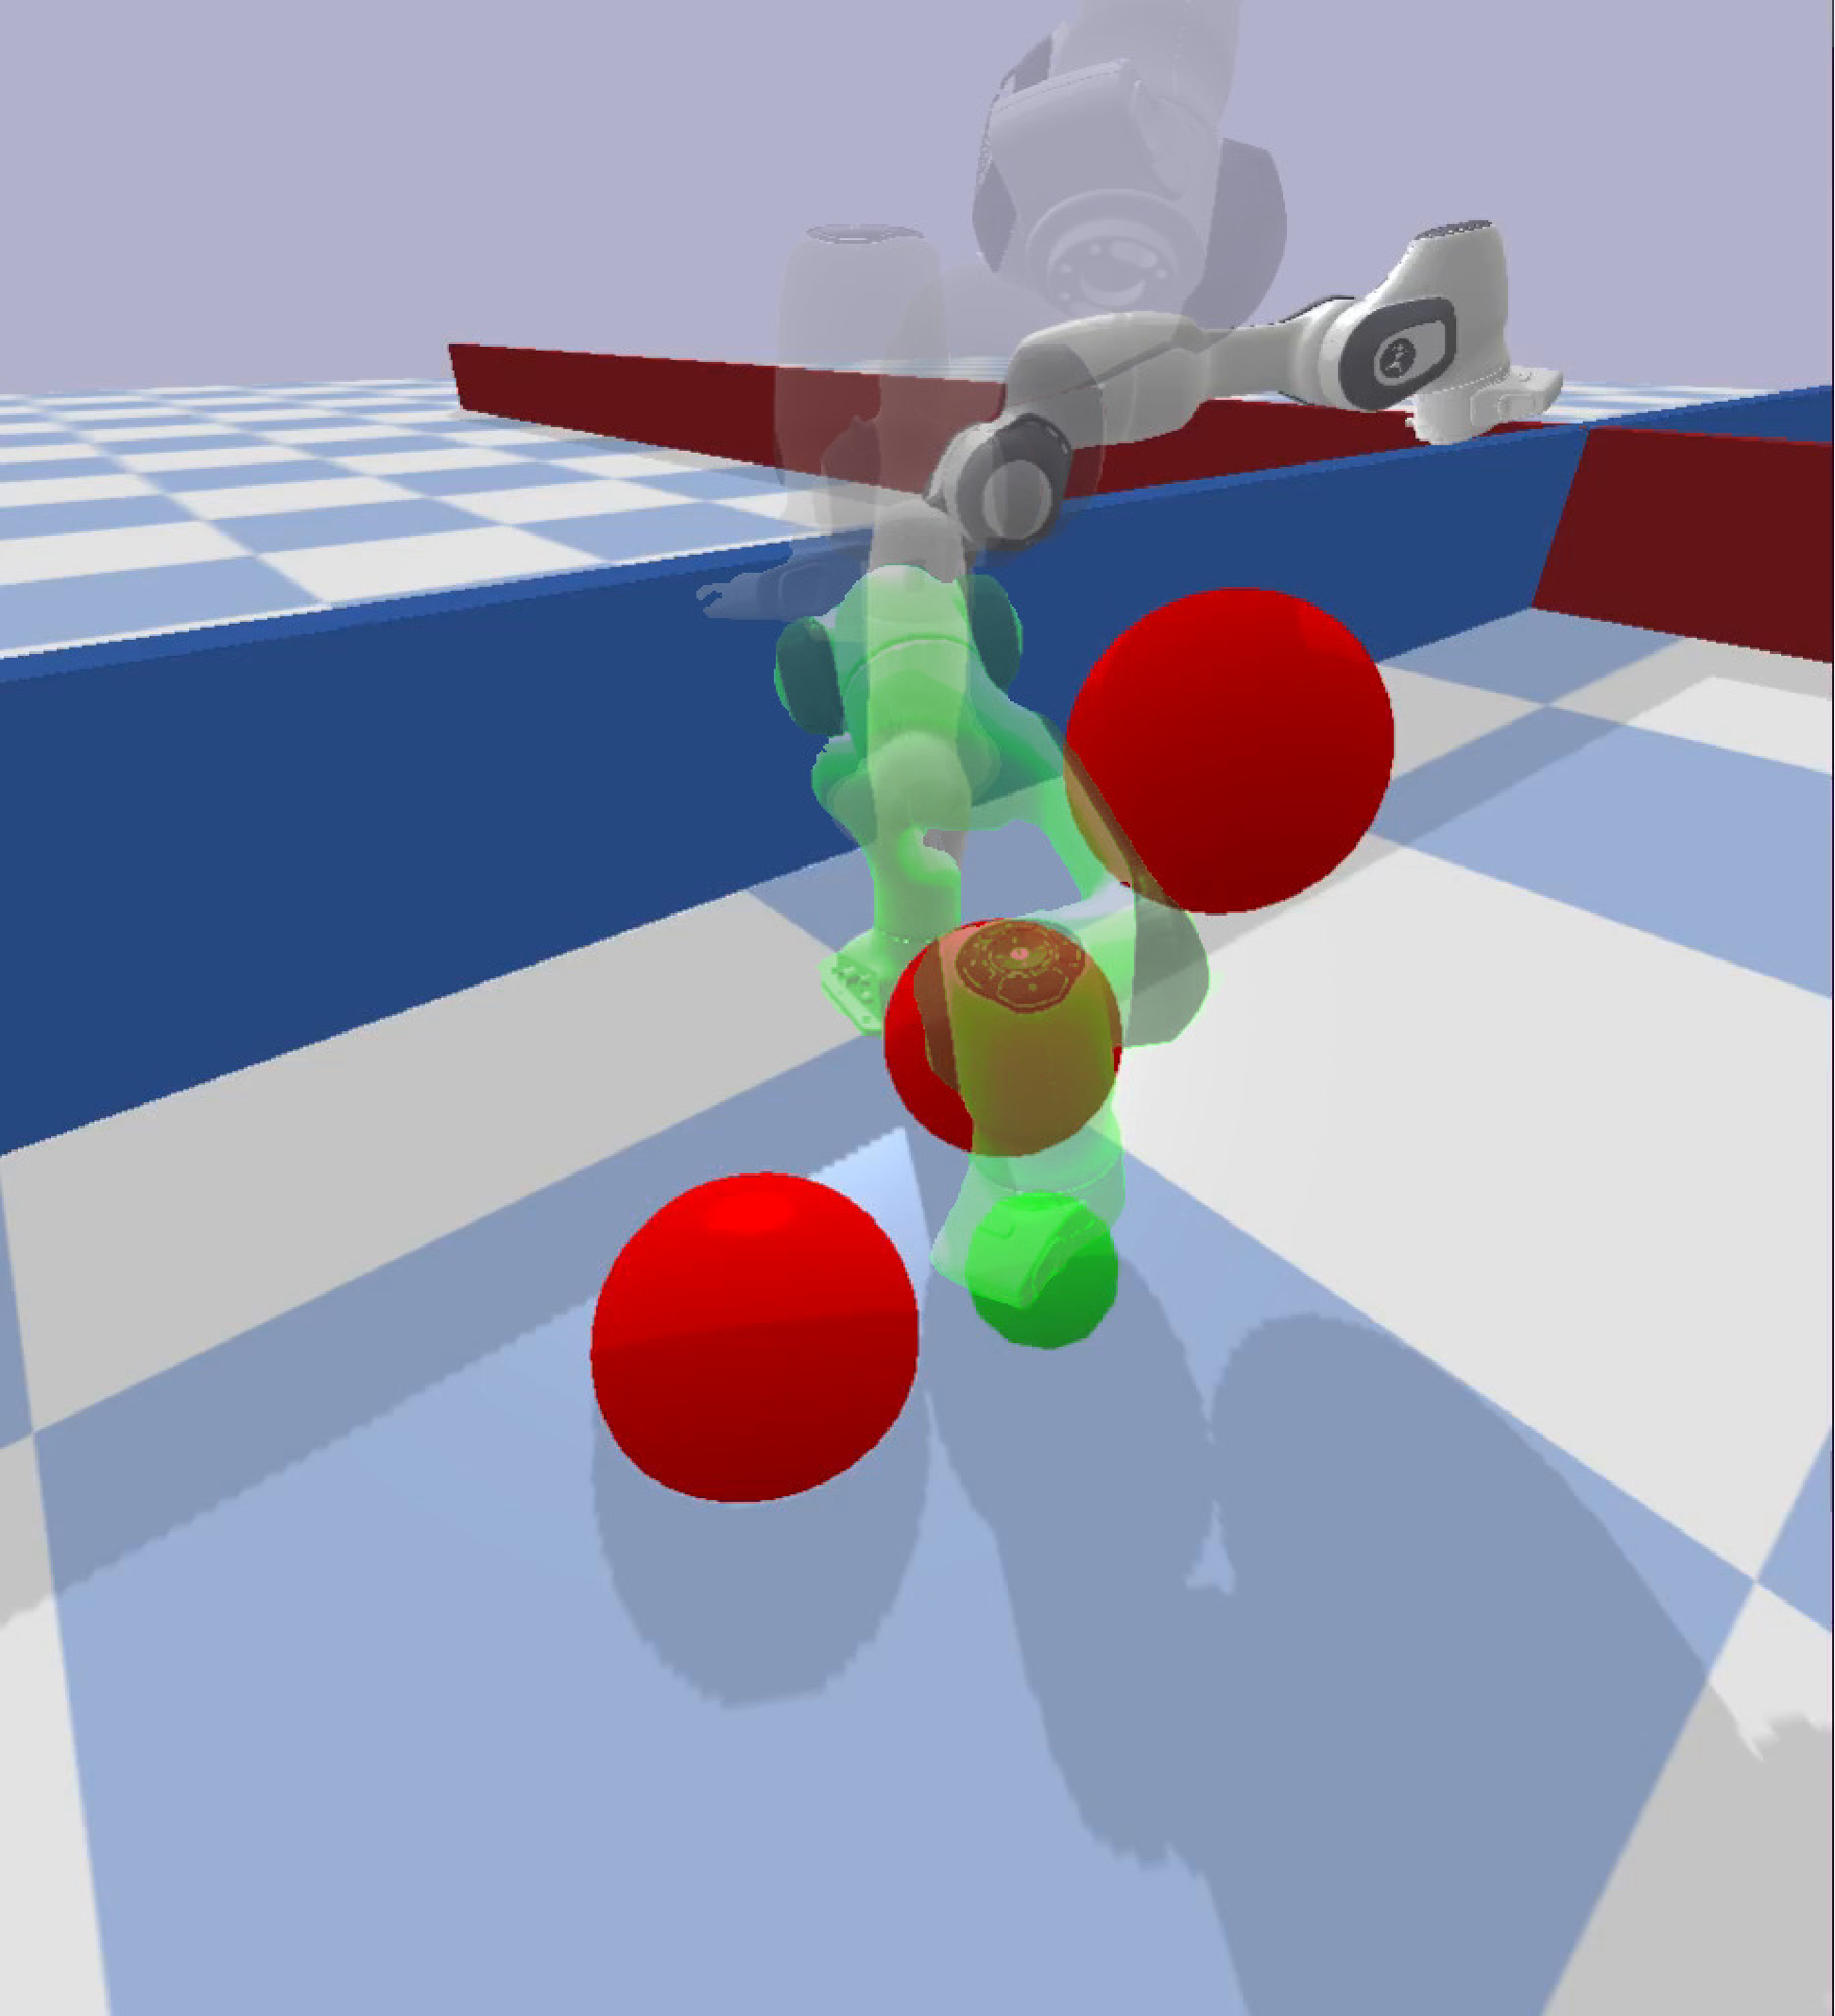
\includegraphics[height=4cm]{1_fabric_mpc/simPanda/fabric_20220223_102405_motion_in_frame}
    \caption{}%
    \label{subfig:experiment1_example}
  \end{subfigure}%
  \begin{subfigure}{0.6\linewidth}
    \centering
    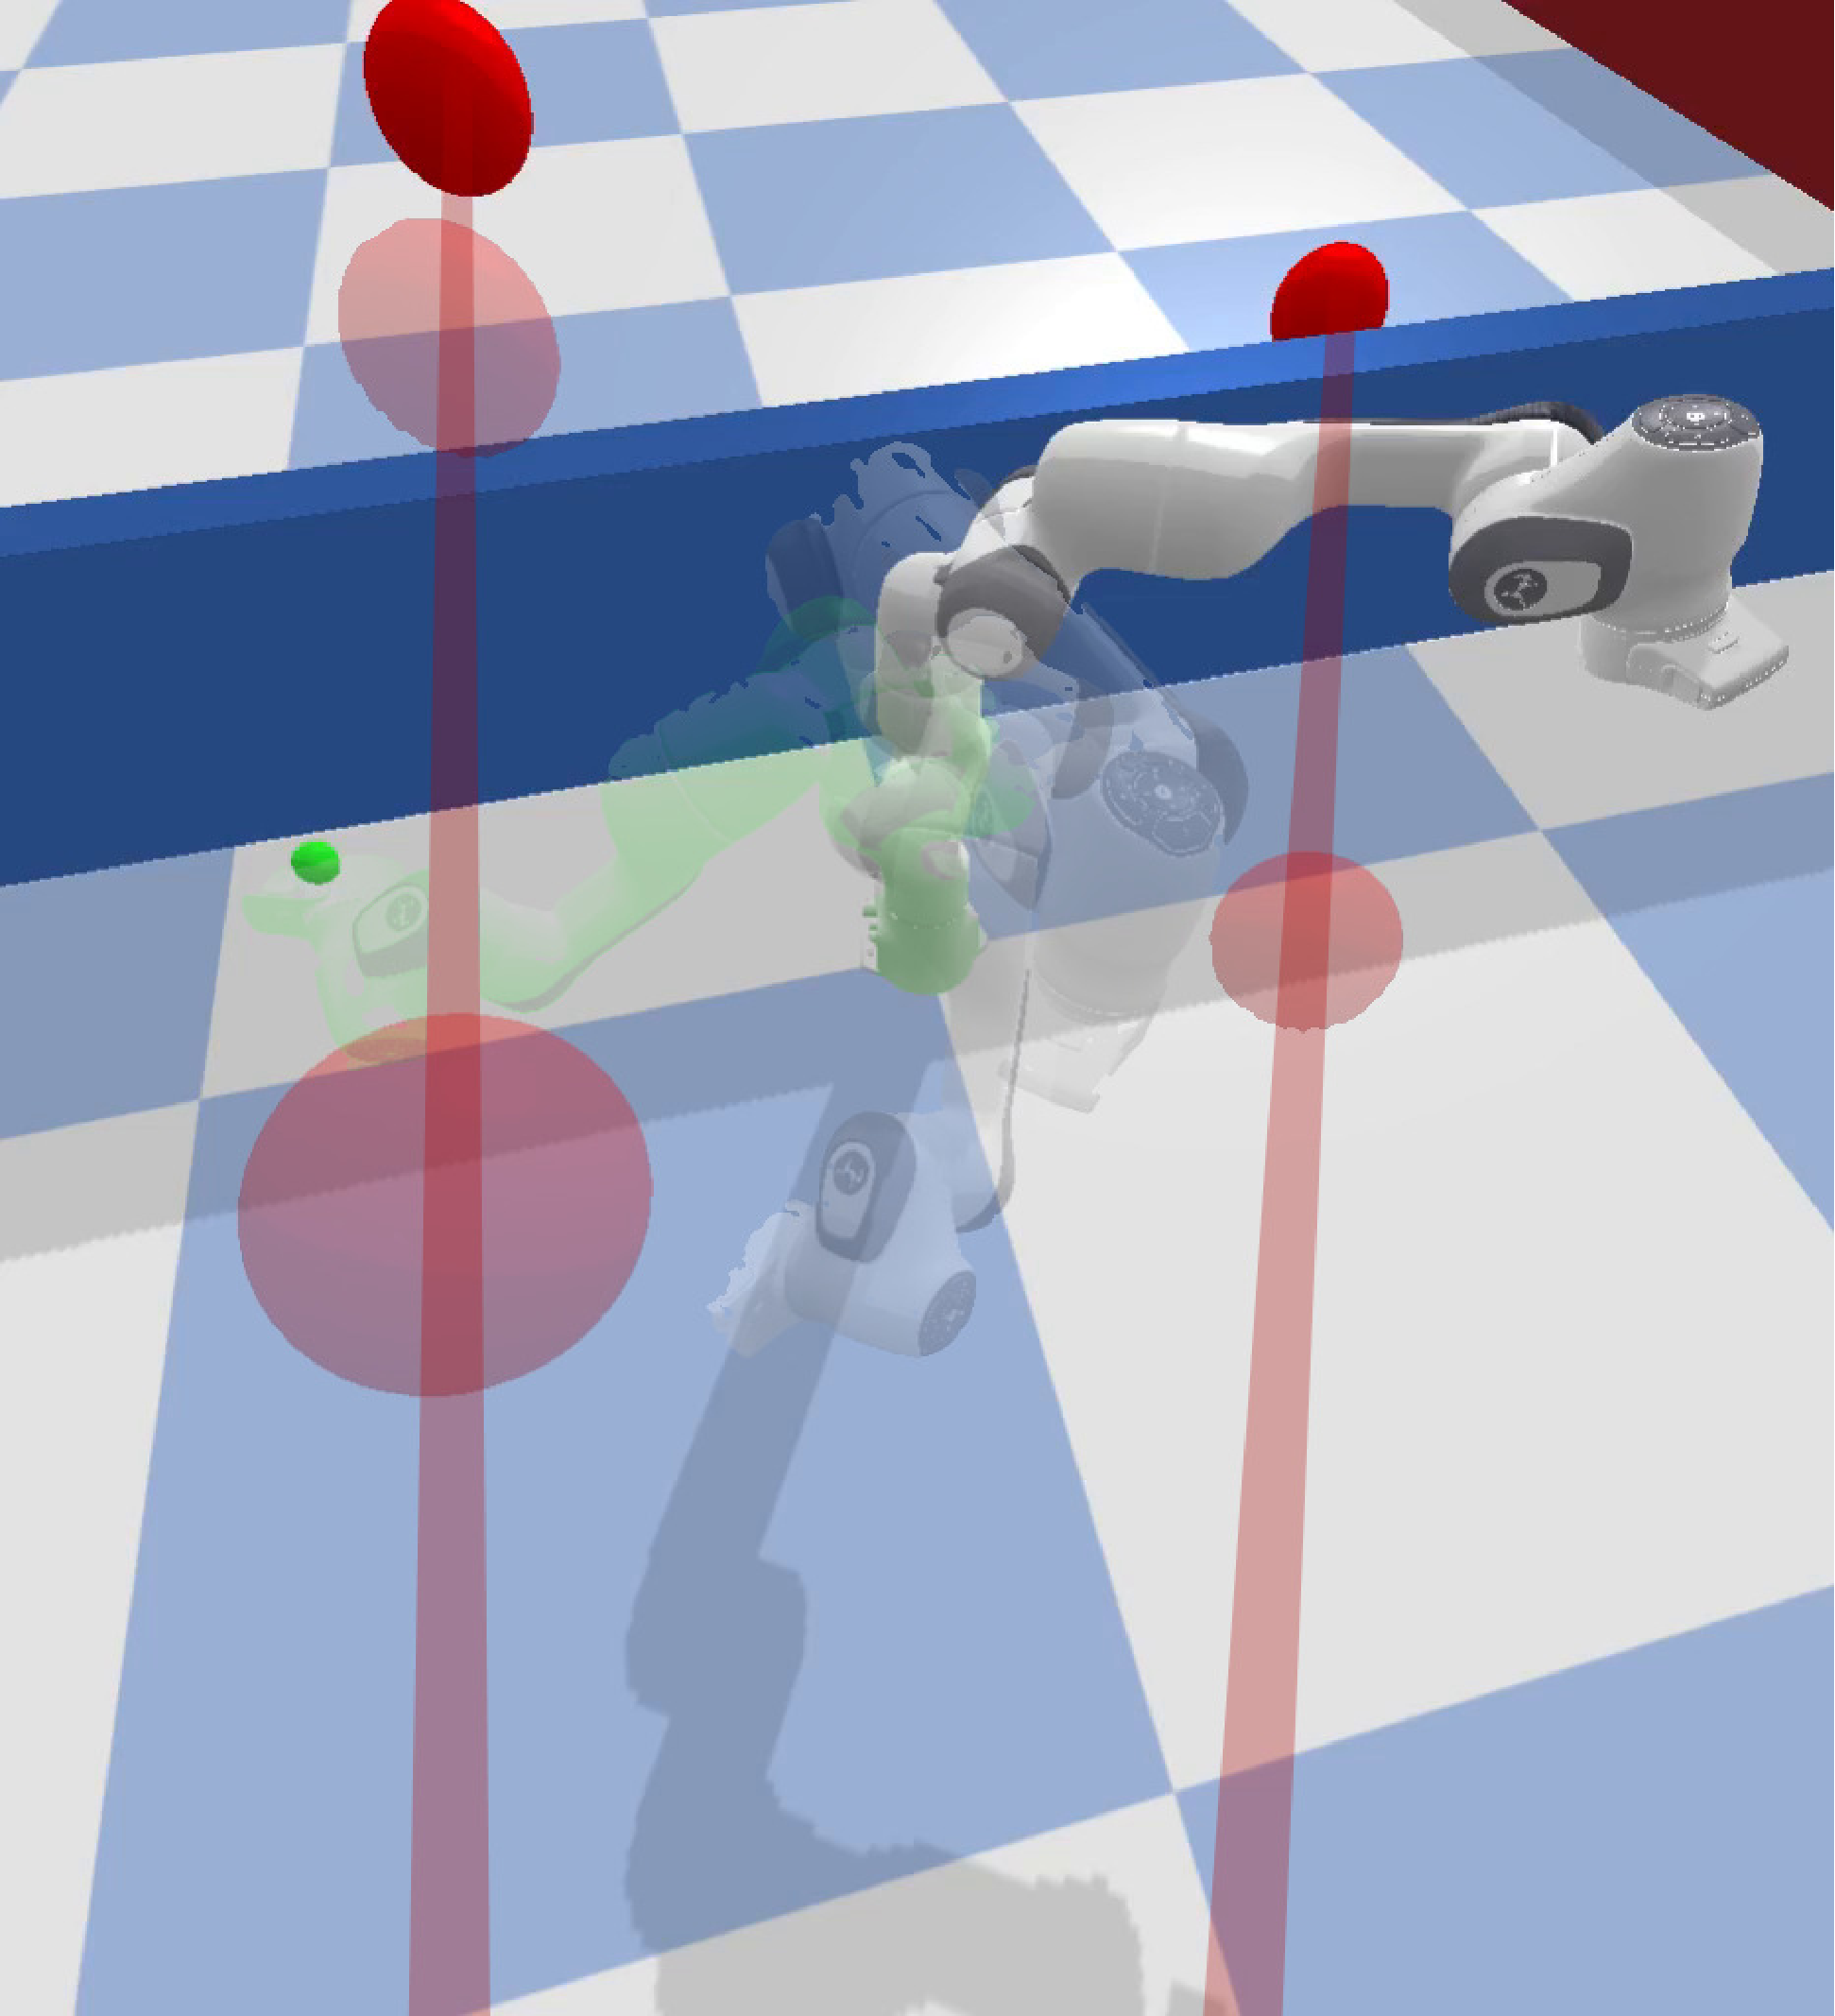
\includegraphics[height=4cm]{3_moving_obstacles/simPanda/dynamicFabric_20220223_102854_motion_in_frame}
    \caption{}%
    \label{subfig:experiment3_example}
  \end{subfigure}
  \caption{Examples for simulation setups with \panda{}.
    Initial configuration are shown in white and final configurations in light green.
    Obstacles are visualized in red. In (a), only static obstacles are considered. In (b),
    the trajectories of two moving obstacles are visualized in light red.
  }%
  \label{fig:experiments_example}
\end{figure}

\paragraph{Simulation}
A series of $N=50$ runs was evaluated with the \panda{} in simulation. Randomized
end-effector positions were set for every run, while the initial configuration
remained unchanged. One to five spherical obstacles of
radius $r=0.15$ m were
placed in the workspace at random. An example setup is shown in
\cref{subfig:experiment1_example}. The results are summarized in 
\cref{fig:experiment1_simPanda}. Solver times with fabrics averaged at $1$ ms while the
\ac{mpc} solver took around $50$ ms in every time step. Although the path length is similar
with both solvers, the minimum clearance from obstacles is increased with \ac{sf}
($0.183$ m) compared to \ac{mpc} ($0.138$ m). This means that the trajectories are
safer and thus more suitable for dynamic environments.
Both motion generation methods fail in 6 cases. However, the \ac{sf} produce only
one collision while \ac{mpc} creates 5 collisions. The remaining failures are deadlocks.
For both methods, deadlocks result from local minima, highlighting the 
need for supportive global plans. Collisions are caused
by numerical inaccuracies, which are generally higher with \ac{mpc} due
to the lower frequency.

\begin{figure}[h]
  \centering
  \begin{subfigure}{1.0\linewidth}
    \centering
    \includegraphics[angle=-90,width=\textwidth]{1_fabric_mpc/simPanda/results_comparison}
    \caption{Metrics evaluation for successful experiments}%
    \label{subfig:experiment1_simPanda_res}
  \end{subfigure}
  \begin{subfigure}{1.0\linewidth}
    \centering
    \includegraphics[angle=-90,width=\textwidth]{1_fabric_mpc/simPanda/success}
    \caption{Success results}%
    \label{subfig:experiment1_simPanda_success}
  \end{subfigure}
  \caption{Results for randomized motion planning problems with the \panda{} in simulation.
    Lower values represent an improved performance of \ac{sf} over MPC.
    %Trajectory computed with optimization fabrics are more conservative and
    %computed in a decreased solver time.
  }%
  \label{fig:experiment1_simPanda}
\end{figure}

\paragraph{Real World}
For the experiments with the real robot, we limited the number of test runs to $N=20$. In
contrast to the simulated results, \ac{mpc} has significantly more collisions than
\ac{sf}, \cref{subfig:experiment1_realPanda_success}.  This is likely to be caused by the
lower frequency at which the \ac{mpc} is running. While in simulation the model matches
the actual behaviour perfectly and the time interval between two computations can be
accuratly predicted, more uncertainty in the model is present in the real world. This
leads to prediction errors that cause collisions.  For the collision free cases, the real
world experiments confirm that optimization fabrics tend to be more conservative with
respect to obstacles, see \textit{Clearance} in \cref{subfig:experiment1_realPanda_res}.
Similar to the simulated results, the solving time is reduced by a factor of around $50$
with fabrics. This
allows to run the planner at a higher frequency and thus generating smoother motions.

\begin{figure}[h]
  \centering
  \begin{subfigure}{\linewidth}
    \centering
    \includegraphics[angle=-90,width=\textwidth]{1_fabric_mpc/realPanda/results_comparison}
    \caption{Metrics evaluation for successful experiments}%
    \label{subfig:experiment1_realPanda_res}
  \end{subfigure}
  \begin{subfigure}{\linewidth}
    \centering
    \includegraphics[angle=-90,width=\textwidth]{1_fabric_mpc/realPanda/success}
    \caption{Success results}%
    \label{subfig:experiment1_realPanda_success}
  \end{subfigure}
  \caption{Results for randomized motion planning problems with the real \panda{}.
    \ac{sf} are more conservative around obstacles, improving on safety, while
    reducing the computational cost by a factor of $\approx$ 50.
    As a result of the increased clearance, collisions are more reliably avoided with
    \ac{sf}.
  }%
  \label{fig:experiment1_realPanda}
\end{figure}

\paragraph{Discussion}
The difference in performance (except for solver time) is likely caused by
the different objective metrics. The objective function in the \ac{mpc}
formulation is mainly governed by the Euclidean distance to the goal while
control inputs and velocity magnitude are given a relative small weight.
Avoidance behaviors, such as joint limit avoidance and obstacle avoidance,
are respected through inequality constraints. In contrast, \ac{sf} design the
objective in a purely geometric manner including all avoidance behaviors.
Thus the manifold for the motion is directly altered by the avoidance
behaviors, i.e., the manifold is \textit{bent} \cite{Ratliff2020} so that
the notion of shortest path changes with the addition of obstacles. This
shaping of the manifold leads to improved canvergence compared to the
combination of Euclidean distance objective function and inequality
constraints used with \ac{mpc}.

\subsection{Experiment 2: Static fabrics vs. Dynamic fabrics}%
\label{sub:experiment_2_static_fabrics_vs_dynamic_fabrics}

In motion planning for dynamic environments, global and local planning methods work together
to achieve efficient and safe motion of the robot. However, \ac{sf}
are not designed to follow global paths. Path
following can only be achieved using a pseudo-dynamic approach where the forcing potential
is shifted in every time step without considering the dynamics of the trajectory.
Therefore, we
propose \ac{df} to allow smoother path following tasks, where the speed of
the goal is also considered during execution. 
In this second experiment, we investigate
how \ac{df} compare to \ac{sf} for path following tasks.
Specifically, we show that \ac{df} outperform \ac{sf} when
following a path generated by a global planner.

\paragraph{Simulation}
We evaluated \ac{df} on the \panda{} robot in simulation with an
analytic, time-parameterized curve and a path generated by a global planner, namely RRT
(\cref{fig:experiment2_simPanda_spline_example}).
In the case of the analytic trajectory, the three obstacles were
randomized across all runs. For the experiment with the global planner, the goal position and 
the obstacles were randomized across all runs.
A total of $N=50$ experiments were executed for this
experiment. The reduced summed error for dynamic fabrics verifies the
theoretical finding that dynamic fabrics can follow paths more closely.
The average error over all runs with the
analytic trajectory is $0.0792$m (\ac{df})
and $0.136$m (\ac{sf}), see
\cref{subfig:experiment2_simPanda_res_analytic} for the comparison.
For the spline path generated with RRT, the
average error over all runs is $0.145$m (\ac{df}) and $0.240$m (\ac{sf}), see
\cref{subfig:experiment2_simPanda_res_spline} for the comparison.


\begin{figure}[h]
  \begin{subfigure}{0.5\linewidth}
    \centering
    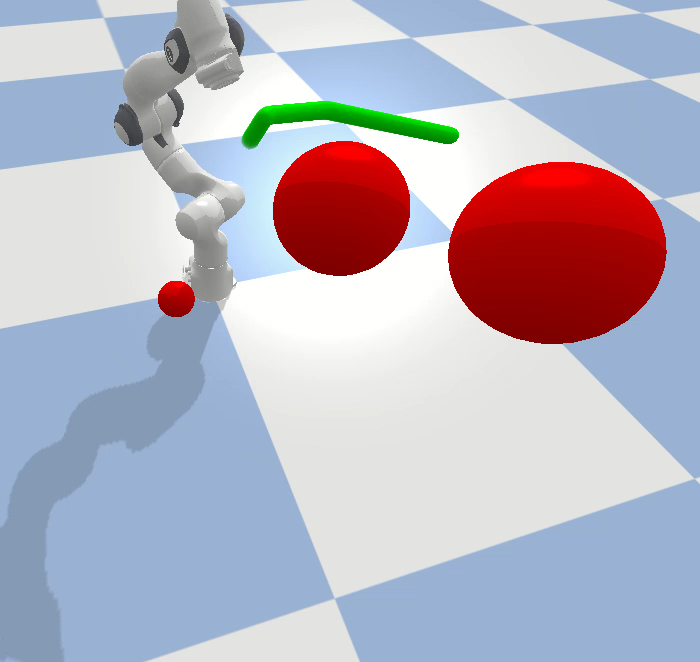
\includegraphics[width=0.95\textwidth]{2_static_dynamic/simPanda/spline/dynamic_fabrics_rrt_1.png}
  \end{subfigure}%
  \begin{subfigure}{0.5\linewidth}
    \centering
    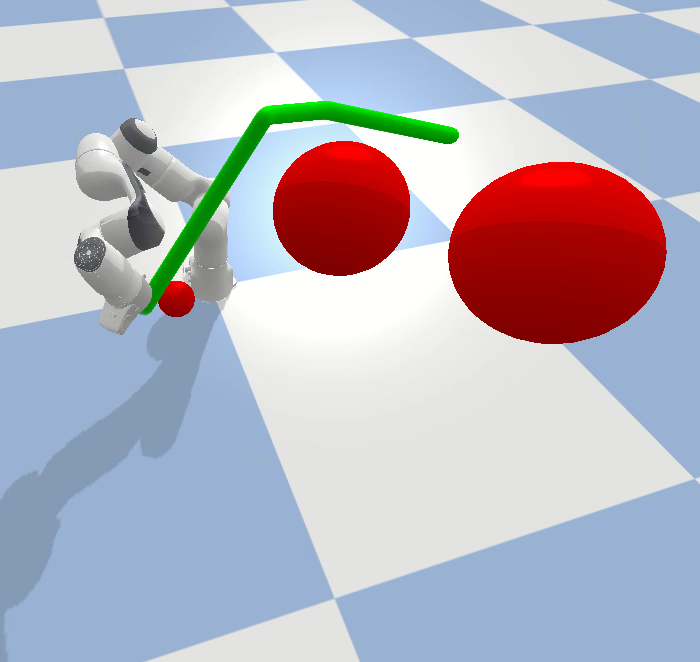
\includegraphics[width=0.95\textwidth]{2_static_dynamic/simPanda/spline/dynamic_fabrics_rrt_2.png}
  \end{subfigure}
  \caption{Path generated with RRT from OMPL.}
  \label{fig:experiment2_simPanda_spline_example}
\end{figure}

\begin{figure}[h]
  \begin{subfigure}{0.5\linewidth}
    \centering
    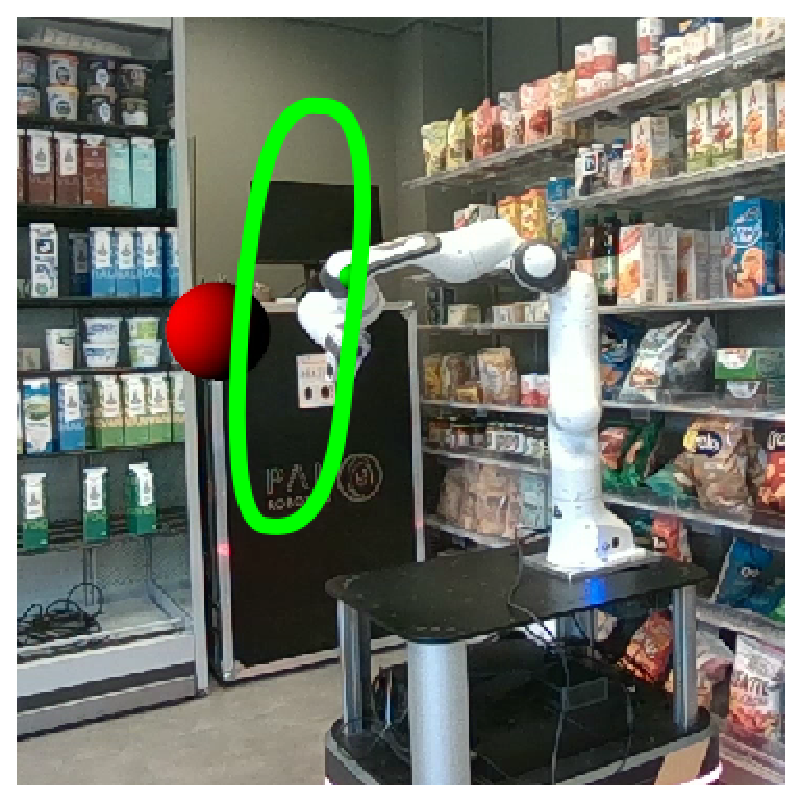
\includegraphics[width=0.95\textwidth]{2_static_dynamic/realPanda/2_static_dynamic_example_analytic}
    \caption{}
  \end{subfigure}%
  \begin{subfigure}{0.5\linewidth}
    \centering
    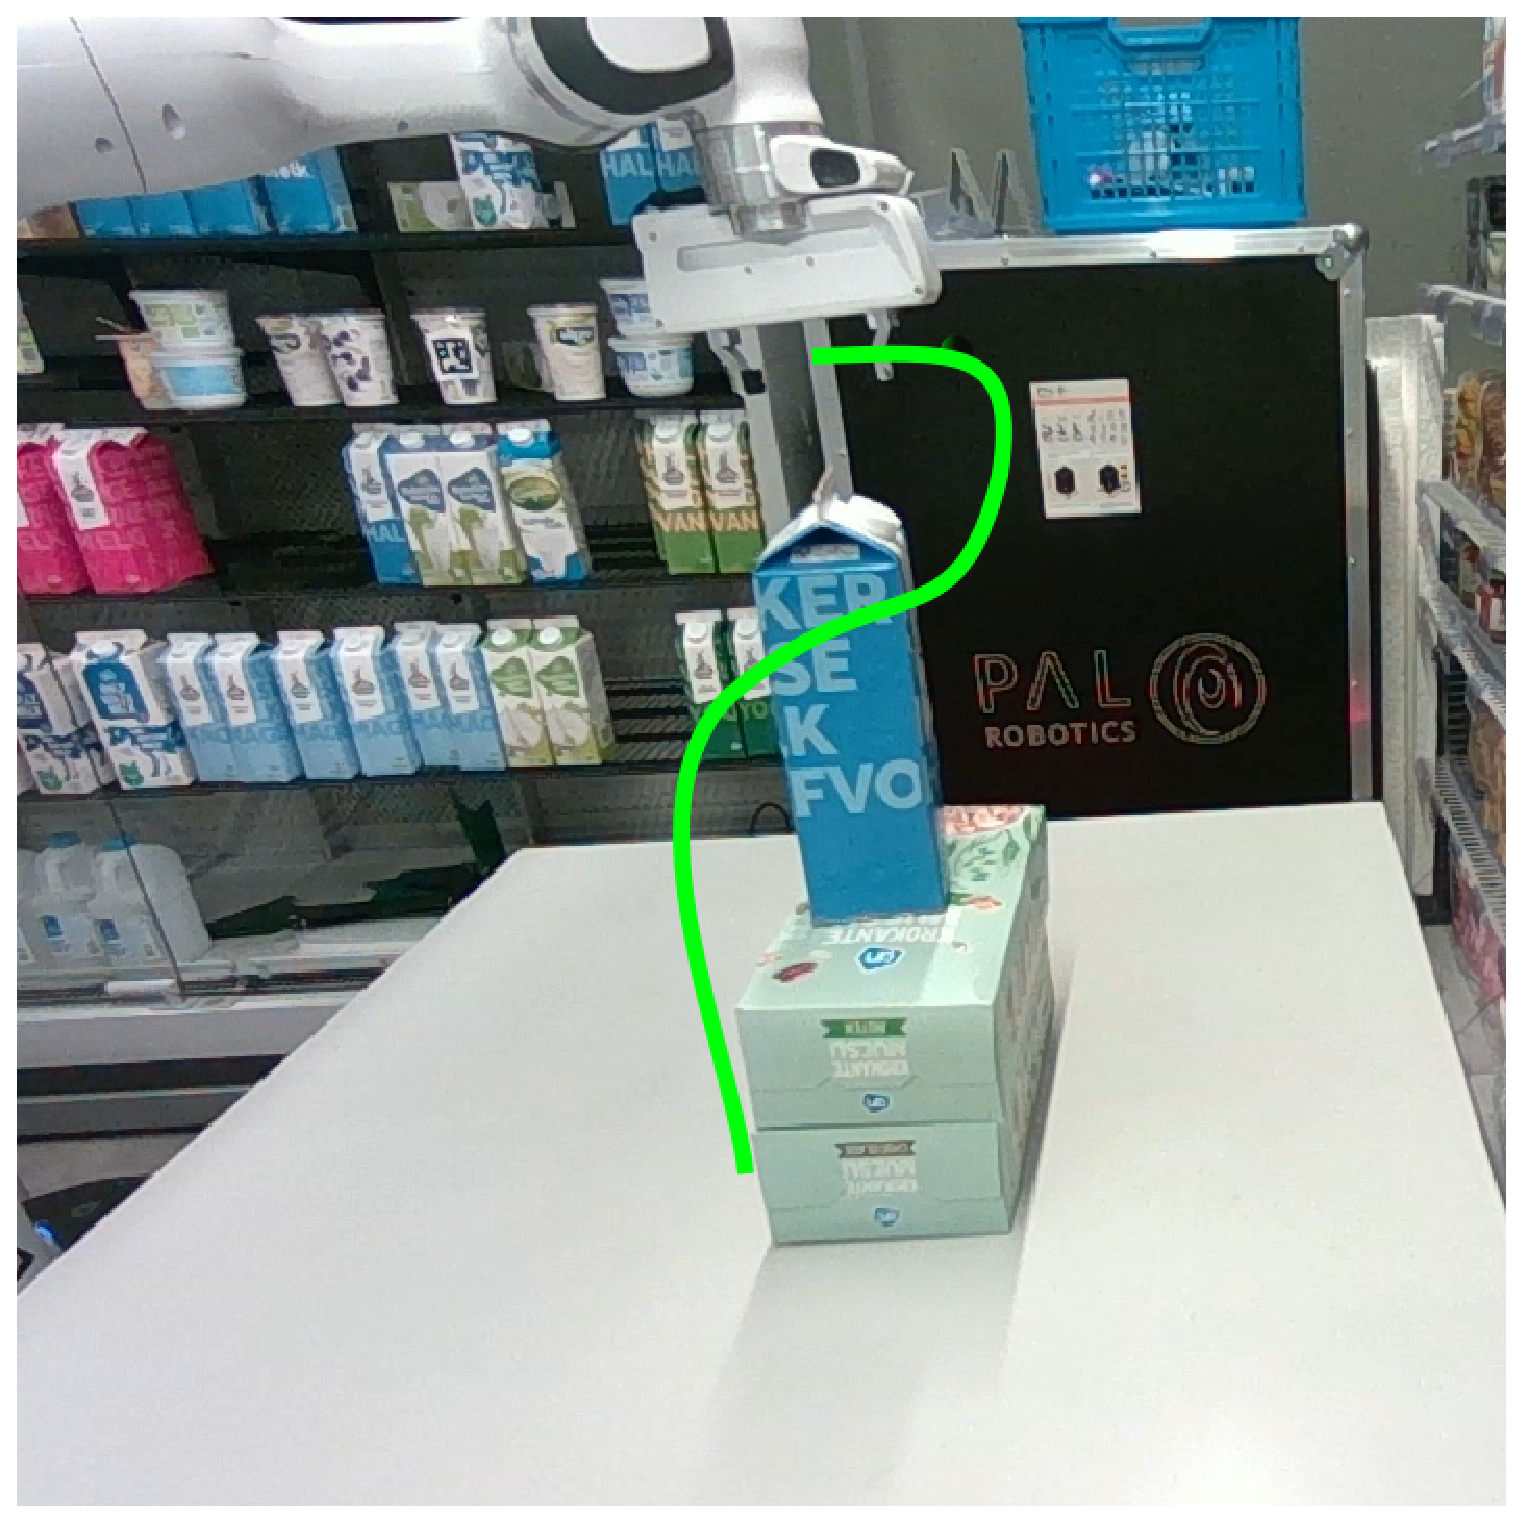
\includegraphics[width=0.95\textwidth]{2_static_dynamic/realPanda/2_static_dynamic_example_spline}
    \caption{}
  \end{subfigure}
  \caption{Trajectory following tasks with \acl{df}. In (a), the trajectory is a 
  time-parameterized analytic curve. In (b), the trajectory is described by a spline.}%
  \label{fig:experiment2_realPanda_examples}
\end{figure}




\begin{figure}[h]
  \centering
  \begin{subfigure}{1.0\linewidth}
    \centering
    \includegraphics[angle=-90,width=\textwidth]{2_static_dynamic/simPanda/analytic/results_comparison}
    \caption{Analytic, user-specified global path}%
    \label{subfig:experiment2_simPanda_res_analytic}
  \end{subfigure}
  \begin{subfigure}{1.0\linewidth}
    \centering
    \includegraphics[angle=-90,width=\textwidth]{2_static_dynamic/simPanda/spline/results_comparison}
    \caption{Global path generated by RRT using OMPL}%
    \label{subfig:experiment2_simPanda_res_spline}
  \end{subfigure}
  \caption{Comparison between static and dynamic fabrics for trajectory following tasks
    in simulation. Lower values in a metric indicate that \ac{df} performed better than
    \ac{sf}.
  }%
  \label{fig:experiment2_simPanda}
\end{figure}

\paragraph{Real-World}
Path following was also assessed with the real \panda{} in similar settings.
Quantitative results are only presented for $N=20$ different paths with splines
where up to three obstacles were added to the workspace, see \cref{fig:experiment2_realPanda_examples}. The results in real-world confirm the 
findings from the simulation. By exploiting the velocity information of the 
trajectory, the integration error can be effectively
reduced, \cref{fig:experiment2_realPanda_res}. In contrast to the simulation
we see a higher fluctuation in solver times, which can be caused by a generally lower capacity 
of the computing unit on the robot.

\begin{figure}[h]
    \centering
    \includegraphics[angle=-90,width=\linewidth]{2_static_dynamic/realPanda/results_comparison}
    \caption{Comparison between \ac{sf} and \ac{df} when following a path defined
      by a basic spline in the real world. 
      The splines and the obstacles are different for the $N=20$ case.
      \ac{df} achieve lower deviation errors that \ac{sf}.
    }%
    \label{fig:experiment2_realPanda_res}
\end{figure}




\subsection{Experiment 3: Moving Obstacles}%
\label{sub:experiment_3_moving_obstacles}
%
Next, we compare the different methods in the presence of dynamic obstacles. All
experiments in this section consist of at least one moving obstacle that follows either an
analytic trajectory or a spline. Here, we use stationary goals to isolate the results from
the behavior investigated in the previous section.

\paragraph{Simulation}
For this series with the simulated \panda{}, 
only the goal position was randomized. The initial configuration 
\[
  \q_0 = {[1.0, 0.0, 0.0, -1.5, 0.0, 1.8675]}^T, 
\]
and the two moving obstacles with the trajectories
\begin{align*}
  \xt_{\textrm{obst1}} &= {[-1.0 + 0.1t, -0.4, 0.7]}^T,  \\
  \xt_{\textrm{obst2}} &= {[-1.0 + 0.2t, 1.0 - 0.1t, 0.3]}^T
\end{align*}
were kept constant throughout all experiments. The environment is visualized in
\cref{subfig:experiment3_example}. The comparison between \ac{sf} and \ac{df}
shows that \ac{df} are more conservative in terms of collision avoidance with
dynamic obstacles. Specifically, the distance between the robot and the
obstacles is increased (\cref{subfig:experiment3_simPanda_res}).
The success rate with \ac{df} compared to \ac{sf} is significantly improved,
see \cref{subfig:experiment3_simPanda_success}. Thus showing the need for
using \ac{df} in dynamic environments.
%
\begin{figure}[ht]
  \centering
  \begin{subfigure}{1.0\linewidth}
    \centering
    \includegraphics[angle=-90,width=\textwidth]{3_moving_obstacles/simPanda/results_comparison}
    \caption{Metrics evaluation for sucessful experiments}%
    \label{subfig:experiment3_simPanda_res}
  \end{subfigure}
  \begin{subfigure}{1.0\linewidth}
    \centering
    \includegraphics[angle=-90,width=\textwidth]{3_moving_obstacles/simPanda/success}
    \caption{Success results}%
    \label{subfig:experiment3_simPanda_success}
  \end{subfigure}
  \caption{Comparison between \ac{sf} and \ac{df} for scenarios with dynamic obstacles.
    While path length and solver time is not increased, clearance is increased and
    the time to reach the goal is reduced with \ac{df} compared to \ac{sf}.
  }%
  \label{fig:experiment3_simPanda}
\end{figure}
%
\paragraph{Real-World}
In a series of $N=20$ experiments, performance on the real panda arm was assessed. The same
trend for more conservative behavior with \ac{df} compared to \ac{sf} can be observed,
\cref{fig:experiment3_realPanda}. However, \ac{df} take longer on average to reach the
goal as they keep larger clearance from obstacles. Note that collisions are effectively
eliminated with \ac{df} compared to \ac{sf}.

\begin{figure}[ht]
  \centering
  \begin{subfigure}{1.0\linewidth}
    \centering
    \includegraphics[angle=-90,width=\textwidth]{3_moving_obstacles/realPanda/results_comparison}
    \caption{Metrics evaluation for successful experiments}%
    \label{subfig:experiment3_realPanda_res}
  \end{subfigure}
  \begin{subfigure}{1.0\linewidth}
    \centering
    \includegraphics[angle=-90,width=\textwidth]{3_moving_obstacles/realPanda/success}
    \caption{Success results}%
    \label{subfig:experiment3_realPanda_success}
  \end{subfigure}
  \caption{Comparison between \ac{sf} and \ac{df} for real-world scenarios with dynamic obstacles.
  }%
  \label{fig:experiment3_realPanda}
\end{figure}


By investigating one example out of the series, see trajectories in
\cref{fig:experiment3_realPanda_example}, the reason for the large number of collisions
with \ac{sf} can be explained.
Both methods initially drive
the end-effector to the goal position. As the moving obstacle is approaching the robot,
the \ac{df} are starting to react while \ac{sf} are not changing its behavior resulting
in a very sudden motion at around $t=30$s.
\ac{sf} treat moving obstacles as pseudo-static (i.e., the position of the obstacle
is updated at every time step, but the information on its velocity is discarded).  As a
result, the relative velocity between obstacle and robot is only a function of the
velocity of the robot. Geometries and energies for collision avoidance with fabrics are,
by design, a function of this velocity and therefore fail to avoid moving obstacles when
the robot moves slowly or not at all. This behavior is most visible when the goal has
already been reached but an obstacle is approaching. \ac{df} on the other hand
take the velocity of the moving obstacles into account and can therefore avoid them.

\begin{figure}[ht]
  \centering
  \begin{subfigure}{0.5\linewidth}
    \centering
    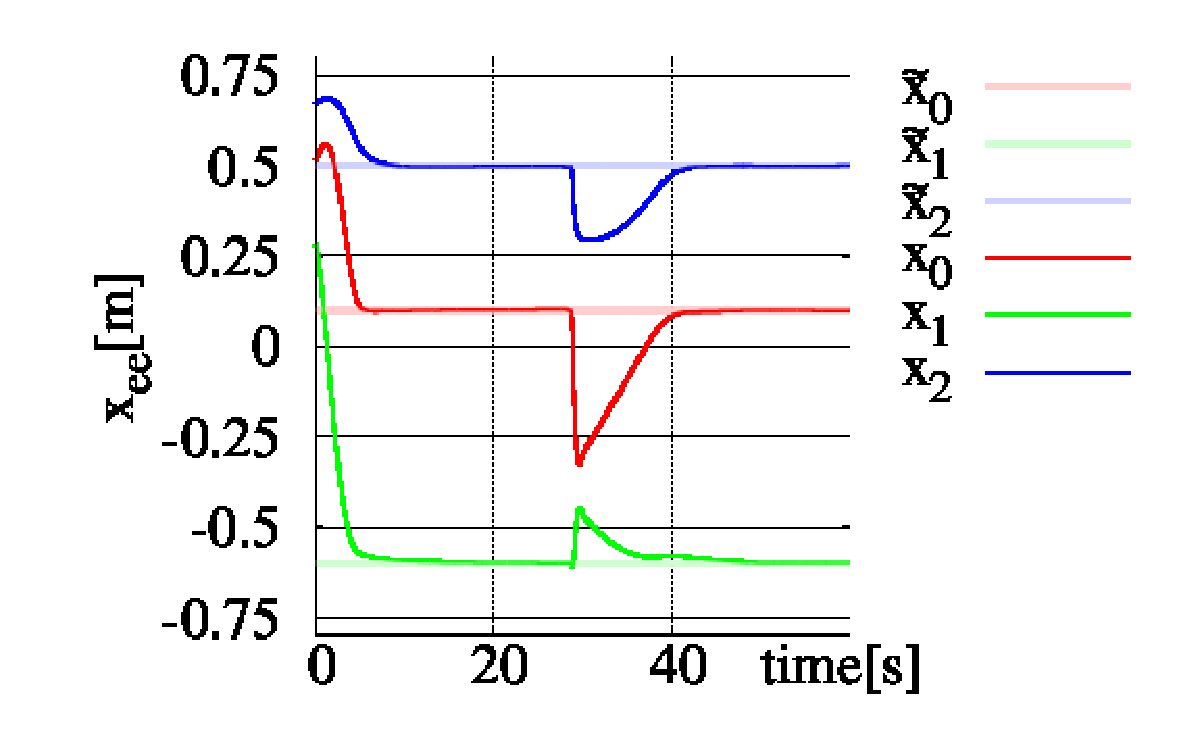
\includegraphics[width=1.\textwidth]{3_moving_obstacles/realPanda/trajectory_static}
    \caption{Static Fabric}%
    \label{subfig:experiment3_realPanda_trajectory_static}
  \end{subfigure}%
  \begin{subfigure}{0.5\linewidth}
    \centering
    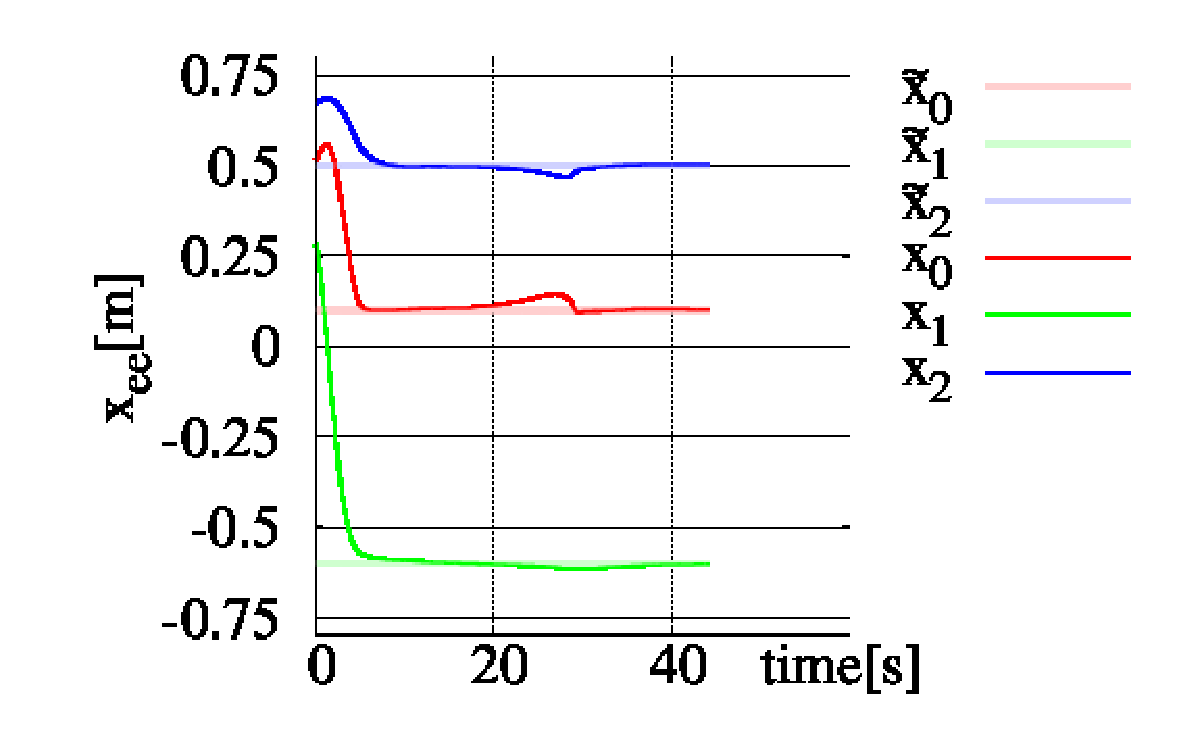
\includegraphics[width=1.\textwidth]{3_moving_obstacles/realPanda/trajectory_dynamic}
    \caption{Dynamic Fabric}%
    \label{subfig:experiment3_realPanda_trajectory_dynamic}
  \end{subfigure}
  \caption{Trajectories for real panda robot in the presence of a dynamic obstacle. \ac{df}
    show a smoother and in-advance reaction to the approaching obstacle
    while \ac{sf} can only react in sudden motion.
  }%
  \label{fig:experiment3_realPanda_example}
\end{figure}

\iffalse%
\MS{Takeaway Experiment3: Only dynamic fabrics are able to respect dynamic obstacles.}
\fi



\subsection{Experiment 4: Nonholonomic robots}%
\label{sub:experiment_4_nonholonomic_robots}

\paragraph{Simulation}
This experiment assesses the performance of the proposed method to compute
trajectories for non-holonomic robots with fabrics. Specifically, we run
experiments for a \textit{Clearpath Boxer} for position. As
for the first experiment, we compare the performance to \ac{mpc}. In this
experiment, the initial position, the goal location, and the position of five
obstacles were randomized. The results reveal that our extension of
optimization fabrics to non-holonomic robots maintains similar results as with
a robotic arm. Specifically, computational time can be reduced to
optimization-based methods while maintaining good performance in terms of
safety and goal-reaching, \cref{fig:experiment4_simBoxer}. We can also observe
that success rate with \ac{sf} is lower compare to \ac{mpc} due to a high
number of unreached goals.

\begin{figure}[h]
  \centering
  \begin{subfigure}{1.0\linewidth}
    \centering
    \includegraphics[angle=-90,width=\textwidth]{4_non_holonomic/simBoxer/results_comparison}
    \caption{Metrics evaluation for successful experiments}%
    \label{subfig:experiment4_simBoxer_res}
  \end{subfigure}
  \begin{subfigure}{1.0\linewidth}
    \centering
    \includegraphics[angle=-90,width=\textwidth]{4_non_holonomic/simBoxer/success}
    \caption{Success results}%
    \label{subfig:experiment4_simBoxer_success}
  \end{subfigure}
  \caption{Results for randomized cased with the Clearpath Boxer robot.
    Similar performance in terms of safety and goal-reaching can be combined with very
    fast computation using optimization fabrics.
  }%
  \label{fig:experiment4_simBoxer}
\end{figure}



\subsection{Experiment 5: Mobile manipulators}%
\label{sub:experiment_5_mobile_manipulators}

In the final experiment, we assess the applicability of \ac{sf} and \ac{df} to a 
non\hyp{}holonomic mobile manipulator. In an environment that is densely occluded by obstacles,
the motion planning problem is defined by a desired end-effector position and additional
path constraints (e.g. desired orientation of the end-effector).
\paragraph{Simulation}
In simulation, we evaluate the performance of our extension to non\hyp{}holonomic
mobile manipulators with \ac{sf}. In this series, the positions of 8 obstacles
are randomized for $N=50$ cases. The workspace was limited to a
7mx7m square, so that random obstacles are ensured to be actually hindering the
motion planner. The results reveal that properties shown in the previous
experiments transfer to more complex systems without loss of the computational
benefit, \cref{fig:experiment5_simAlbert_results}. In this series, there were
1 unreached goals and 4 collisions which are, similar
to the previous experiments, caused by local minima. Local minima are more
likely for mobile manipulators as their workspace is larger.
%
\begin{figure}[ht]
  \centering
  \begin{subfigure}{1.0\linewidth}
    \centering
    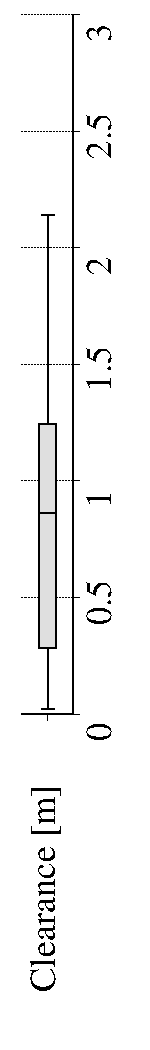
\includegraphics[angle=-90,width=\textwidth]{4_non_holonomic/simAlbert/results_fabric_clearance}
  \end{subfigure}
  \begin{subfigure}{1.0\linewidth}
    \centering
    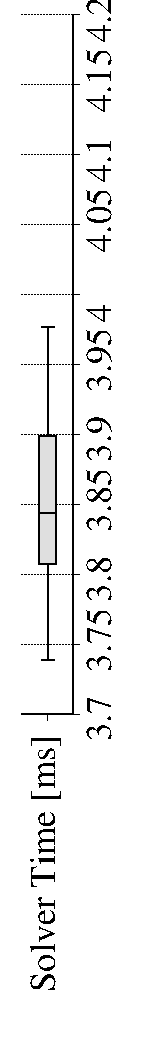
\includegraphics[angle=-90,width=\textwidth]{4_non_holonomic/simAlbert/results_fabric_solverTime}
  \end{subfigure}
  \begin{subfigure}{1.0\linewidth}
    \centering
    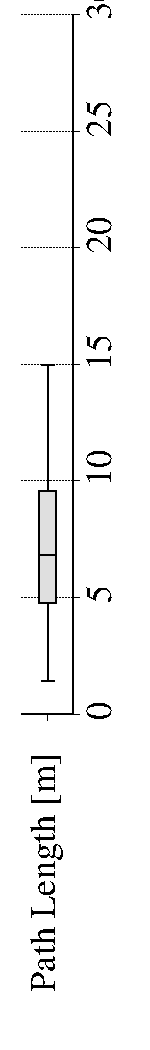
\includegraphics[angle=-90,width=\textwidth]{4_non_holonomic/simAlbert/results_fabric_pathLength}
  \end{subfigure}
  \begin{subfigure}{1.0\linewidth}
    \centering
    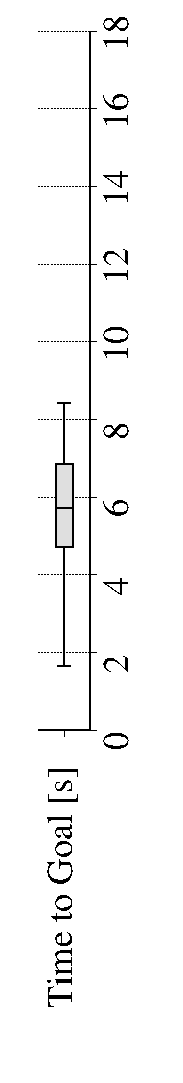
\includegraphics[angle=-90,width=\textwidth]{4_non_holonomic/simAlbert/results_fabric_time2Goal}
  \end{subfigure}
  \begin{subfigure}{1.0\linewidth}
    \centering
    \includegraphics[angle=-90,width=\textwidth]{4_non_holonomic/simAlbert/success}
  \end{subfigure}
  \caption{Quantitative results with static fabrics for a 
    non\hyp{}holonomic mobile manipulator in simulation. Fabrics solve planning problems in
    randomized environments in low planning time. This allows whole-body control and highly
    reactive behavior.
  }%
  \label{fig:experiment5_simAlbert_results}
\end{figure}
%
Combining our contributions, \ac{df} and the extension to non\hyp{}holonomic robots, we
achieve reactive and safe behavior in dynamic environments. Moving obstacles are avoided in a natural way
using our method, see \cref{fig:albert_moving_obstacles}.
%
\begin{figure*}
  \centering
  \begin{subfigure}{.2\linewidth}
    \centering
    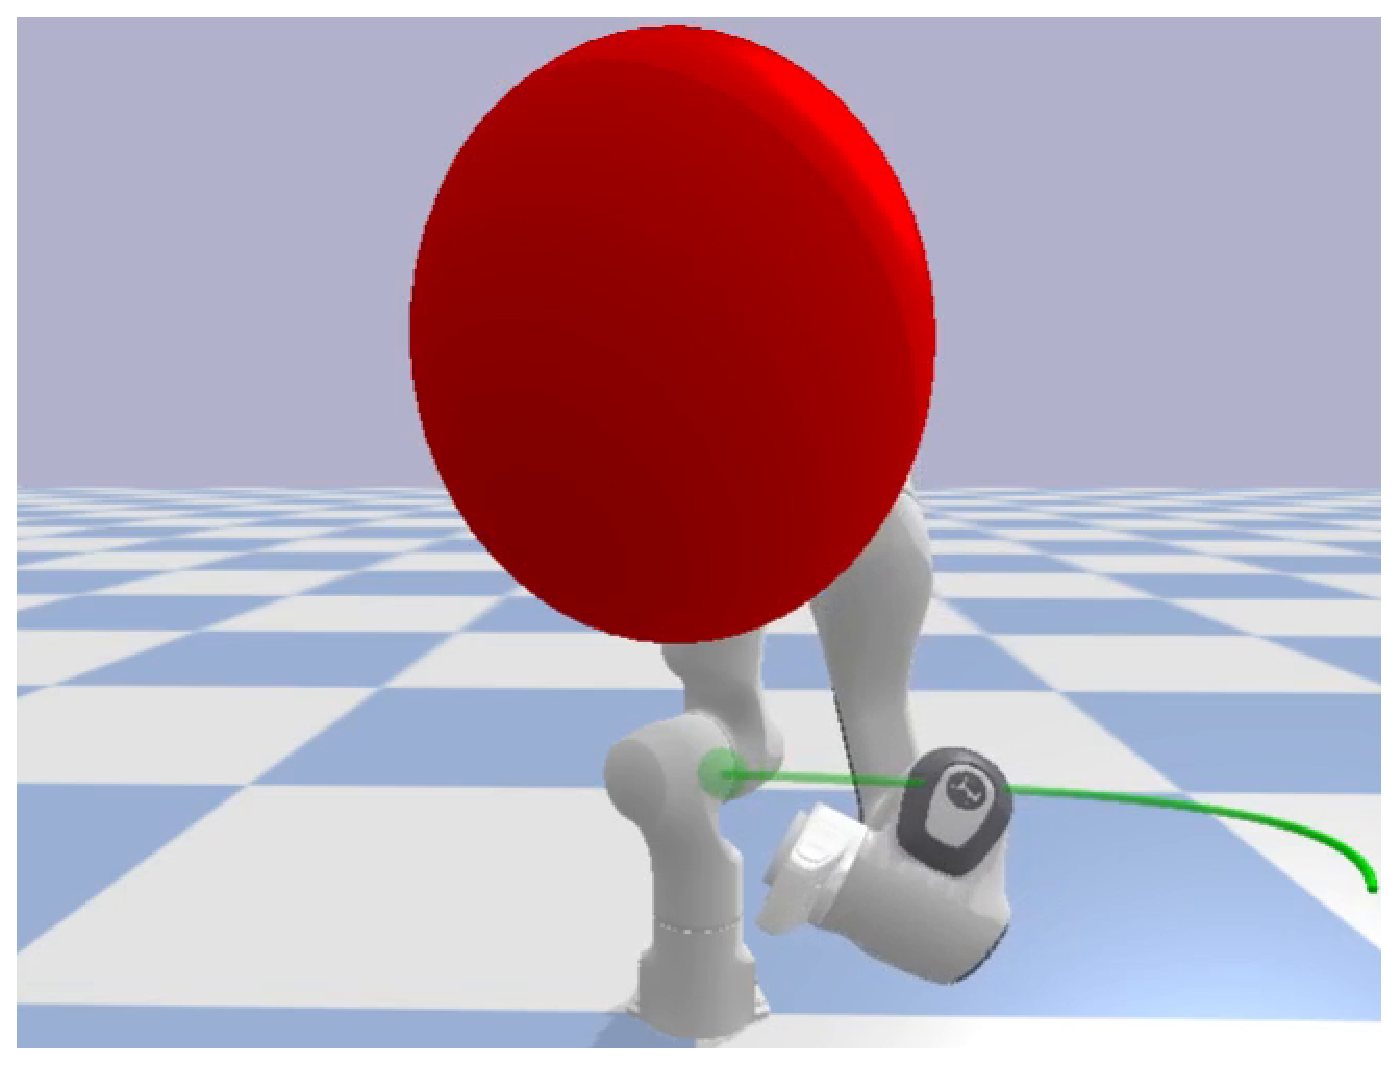
\includegraphics[width=0.9\linewidth]{4_non_holonomic/simAlbert/example_1}
  \caption{$t=0$s}
  \end{subfigure}%
  \begin{subfigure}{.2\linewidth}
    \centering
    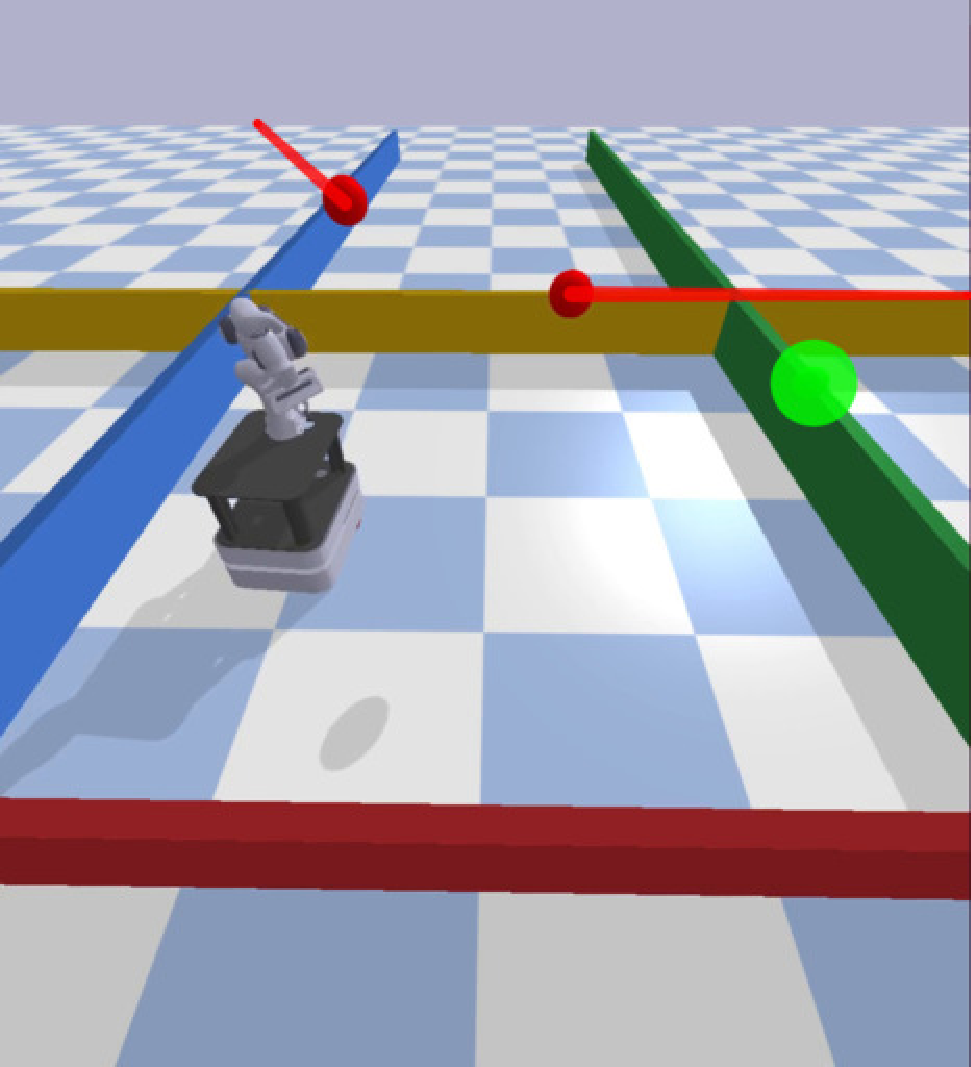
\includegraphics[width=0.9\linewidth]{4_non_holonomic/simAlbert/example_2}
  \caption{$t=7$s}
  \end{subfigure}%
  \begin{subfigure}{.2\linewidth}
    \centering
    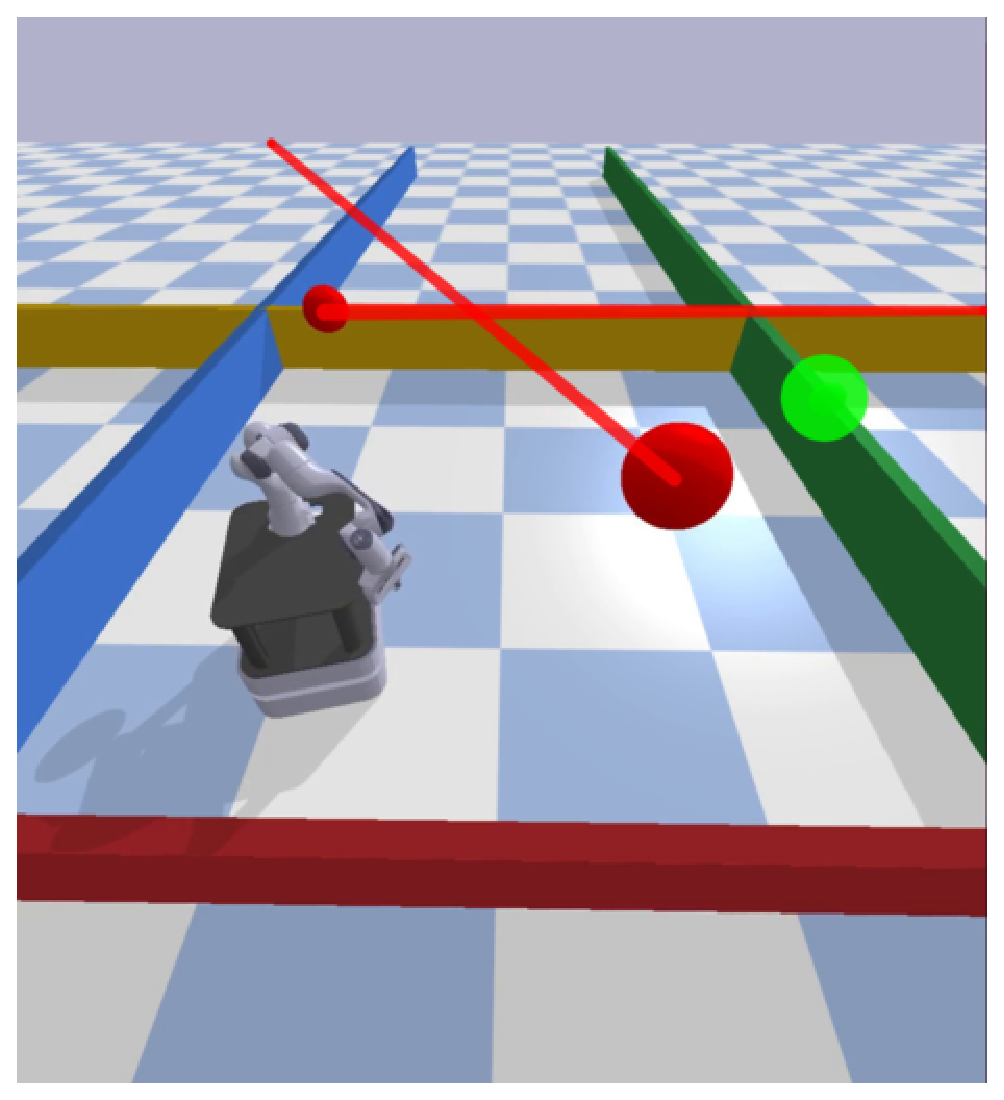
\includegraphics[width=0.9\linewidth]{4_non_holonomic/simAlbert/example_3}
  \caption{$t=14$s}
  \end{subfigure}%
  \begin{subfigure}{.2\linewidth}
    \centering
    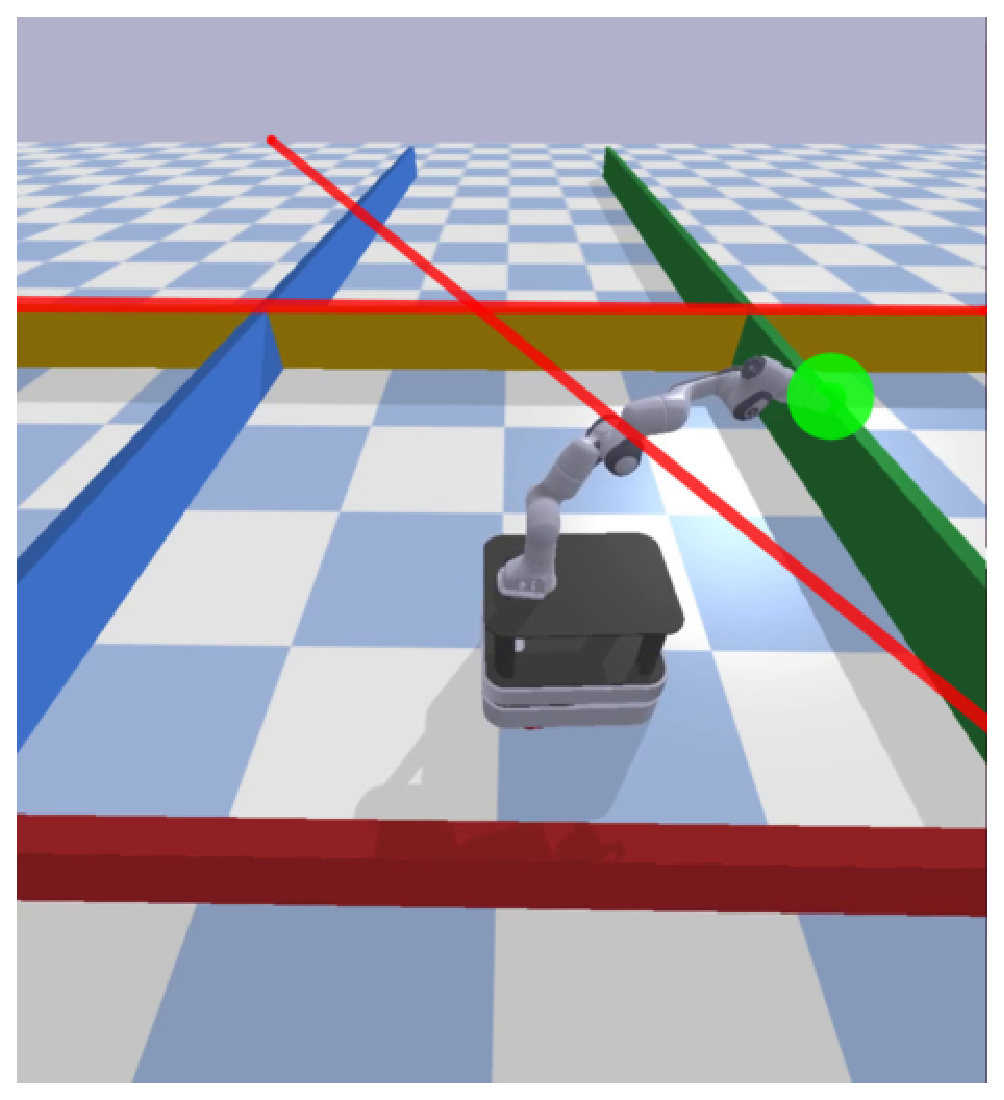
\includegraphics[width=0.9\linewidth]{4_non_holonomic/simAlbert/example_4}
  \caption{$t=20$s}
  \end{subfigure}%
  \begin{subfigure}{.2\linewidth}
    \centering
    \includegraphics[width=1.0\linewidth]{4_non_holonomic/simAlbert/trajectory}
  \caption{}%
  \label{subfig:albert_moving_obstacles}
  \end{subfigure}
  \caption{Sequence of trajectory computed with \ac{df} for a mobile manipulator in simulation with moving obstacles (red sphere with line indicating the past trajectory) and one end-effector goal (green). The trajectory of the end-effector are 
  visualized in (e) as \x{} and the desired end-effector
  position as \xt{}.
  }%
  \label{fig:albert_moving_obstacles}
\end{figure*}
%
\paragraph{Real-World}
We present qualitative results for a non\hyp{}holonomic mobile manipulator using \ac{df}.
In \cref{fig:albert_spline_example}, the robot follows a trajectory defined by a basic spline,
while additionally respecting an orientation constraints on its end-effector and avoiding
the shelves and an obstacle on the ground. The end-effector trajectory is plotted in \cref{fig:albert_spline_trajectory}.
%
\begin{figure}[t!]
    \centering
    \includegraphics[width=0.9\linewidth]{4_non_holonomic/realAlbert/trajectory}
    \caption{Real-world experiment for path following with a mobile manipulator. The global path can be tracked
        accurately by \ac{df} including the extension to non\hyp{}holonomic robots. The scene 
        is visualized in \cref{fig:albert_spline_example}.}
    \label{fig:albert_spline_trajectory}
\end{figure}
%
\iffalse
%
\begin{figure}[ht]
  \centering
  \includegraphics[width=0.8\linewidth]{4_non_holonomic/realAlbert/motion_in_frame}
  \caption{Trajectory following with mobile manipulator. \MS{This needs to be redone \ldots}}%
  \label{fig:albert_trajectory_following}
\end{figure}
%
\fi

\subsection{Experiment 6: Dynamic fabrics in supermarkets}%
\label{sub:experemint_6_dynamic_fabrics_in_supermarkets}
%
In this experiment, we show qualitatively how \ac{df} could be used in
collaborative environments where humans and robots coexist. For this
experiment, we give the robot a static goal pose similar to a pickup setup. The
same environment is shared with a co-worker who restocks a shelf. The right
hand of the human is tracked with a motion capture system.
The hand is then avoided by the robot using \ac{df}, see
\cref{fig:experiment6_realPanda}. In this experiment, the minimum distance
between the robot and the hand was $0.062$m. This real-world experiment
showcases potential applications of the proposed method.

